\documentclass[conference]{IEEEtran}
\IEEEoverridecommandlockouts
% The preceding line is only needed to identify funding in the first footnote. If that is unneeded, please comment it out.
\usepackage[portuguese]{babel} % for dates and expressions as “table of contents”, “chapter” or “appendix” translated
\usepackage[utf8]{inputenc} % for keyboard pt-br
\usepackage{cite}
\usepackage{amsmath,amssymb,amsfonts}
\usepackage[portuguese, ruled, linesnumbered]{algorithm2e}
\usepackage{graphicx}
\usepackage{textcomp}
\usepackage{xcolor}
\def\BibTeX{{\rm B\kern-.05em{\sc i\kern-.025em b}\kern-.08em
    T\kern-.1667em\lower.7ex\hbox{E}\kern-.125emX}}
\begin{document}

\title{Conflito de Transações em Redes Bitcoin\\}

\author{\IEEEauthorblockN{Hellan Dellamycow Gomes Viana}
\IEEEauthorblockA{\textit{Departamento de Ciência da Computação} \\
\textit{Universidade Federal da Bahia}\\
Salvador, Brasil \\
dellamycow@gmail.com}
\and
\IEEEauthorblockN{Patrick Silva Ferraz}
\IEEEauthorblockA{\textit{Departamento de Ciência da Computação} \\
\textit{Universidade Federal da Bahia}\\
Salvador, Brasil \\
patrick.ferraz@outlook.com}
}

\maketitle

\begin{abstract}
Este relatório é parte do trabalho prático da disciplina MATD74 - Algoritmos e Grafos, semestre 2019.1. Nele aborda-se uma proposta de solução para o problema de transações conflitantes em uma rede Bitcoin, utilizando-se do método de Conjuntos Independentes Máximo, que pertence a classe NP-Completo.
\end{abstract}

\begin{IEEEkeywords}
transações, Bitcoin, Conjuntos Independentes, duplo gasto
\end{IEEEkeywords}

\section{Introdução}

Bitcoin é uma nova moeda criptografada disruptiva baseada em um protocolo descentralizado de código aberto que vem gradualmente ganhando força. Apesar de diversos mecanismos associados a segurança e confiabilidade do funcionamento da cadeia de blocos gerada nesse ecossistema, vários tipos de ataques provenientes do problema de gasto duplo surgiram, e por sua vez uma das principais razões para tal fato é a existência de conflitos entre transações na rede Bitcoin. E é com o sentido de tratar as transações conflitantes que este relatório foi idealizado e está sendo apresentado. Nas seções seguintes iremos discutir sobre o Referencial Teórico, Descrição Formal do Problema, Justificativa de o problema ser NP-Completo, Revisão da Literatura e Metodologia.

\section{Referencial Teórico}

\subsection{Transação de Bitcoin}

Transação, no contexto da criptomoeda Bitcoin (BTC),  é uma transferência do valor do BTC que é transmitido para a rede, coletada em blocos, e normalmente fazendo referência a outpus de transações anteriores como novas inputs de transação e dedica todos os valores de BTC de input a novos outputs. As transações tem por característica não serem  criptografadas, permitindo a visualização de todas as transações já coletadas em um bloco. Estando as transações já consolidadas sob confirmações suficientes, elas podem ser consideradas irreversíveis.

Os outpus de transação padrão nomeiam endereços e o resgate de quaisquer inputs futuras requer uma assinatura relevante.

Todas as transações são visíveis na blockchain (ou \emph{cadeia de blocos} em português) e podem ser visualizadas com um editor hexadecimal. Um navegador de blockchain é um site em que todas as transações incluídas na cadeia de blocos podem ser visualizadas em termos legíveis por qualquer pessoa, e possibilitam a leitura dos detalhes técnicos das transações e a verificação dos pagamentos.

A figura \ref{tabela} apresenta o formato generalizado de uma transação Bitcoin dentro de um bloco, trazendo a descrição e tamanhos dos campos. 

\begin{figure}[h]
\centerline{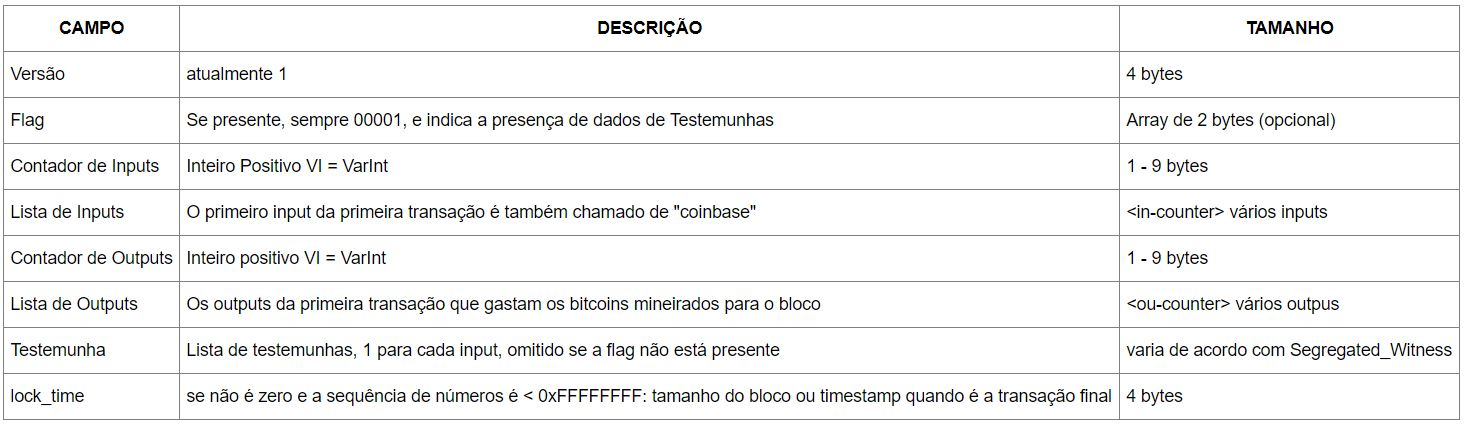
\includegraphics[width=.5\textwidth]{imgs/tabela.JPG}}
\caption{Formato generalizado de uma transação Bitcoin (dentro do bloco).}
\label{tabela}
\end{figure}




\subsection{Como a mineração funciona e as transações são processadas}

O foco desse trabalho não é a mineração de Bitcoin em si, mas as transações (mais especificamente os conflitos entre elas). Contudo, elas estão inseridas no contexto de mineração, e para que se tenha uma melhor observação e conhecimento do processo como todo, sequencialmente é apresentado de forma resumida um passo-a-passo do mecanismo de mineração e como as transações estão intrisecamente inseridas e são processadas. 

\begin{enumerate}
    \item  Um usuário tenta enviar uma certa criptografia ou token para outra pessoa, através de uma carteira;
    
    \item A transação é transmitida pela carteira e agora está esperando em um "conjunto, ou pool, de transações não confirmadas" para ser pego por um minerador no blockchain correspondente.
    
    \item Mineradores na rede, ou nós, selecionam transações desses pools e os formam em um "bloco", que é uma coleção de transações (até então ainda não confirmadas), além de alguns metadados extras. Todo minerador constrói seu próprio bloco de transações, podendo vários mineradores selecionar a mesma transação a ser incluída em seu bloco;
    
    \item Ao selecionar as transações, os mineradores criam um bloco de transações. Para adicionar este bloco de transações ao blockchain (para que todos os outros mineradores e nós registrem as transações), o bloco primeiro precisa de uma assinatura (também chamada de prova de trabalho). Essa assinatura é criada pela solução de um problema matemático muito complexo exclusivo de cada bloco de transações e todos são igualmente difíceis de resolver, sendo necessário poder computacional elevado. Este é o processo conhecido como mineração;
    
    \item O minerador que encontra uma assinatura elegível para o seu bloco primeiro transmite este bloco e a sua assinatura para todos os outros mineradores;
    
    \item Outros mineradores verificam a legitimidade da assinatura pegando a sequência de dados do bloco transmitido e fazendo um hashing para ver se o hash de saída realmente corresponde à assinatura incluída. Sendo válido, os outros mineiros confirmarão sua validade e concordarão que o bloco pode ser adicionado ao blockchain. A assinatura é a "prova" do trabalho realizado (o poder computacional gasto). O bloco agora pode ser adicionado ao blockchain e é distribuído por todos os outros nós da rede. Os outros nós aceitarão o bloco e o salvará em seus dados de transação, desde que as transações dentro do bloco correspondam corretamente aos saldos atuais do histórico de transações naquele momento;
    
    \item Após um bloco ser adicionado à cadeia, todos os outros blocos adicionados em cima agem como uma "confirmação" para esse bloco. Toda vez que outro bloco é adicionado sobre ele, o blockchain alcança o consenso novamente no histórico de transações completo, incluindo sua transação e seu bloco. Quanto mais confirmações a transação tiver, mais difícil será para os invasores alterá-lo. Depois que um novo bloco é adicionado ao blockchain, todos os mineradores precisam selecionar outras transações, formando novos blocos de transações.
\end{enumerate}


\section{Descrição Formal do Problema}
\label{subsec:descricao_formal_do_problema}

As transações, no contexto de Bitcoin, podem eventualmente possuir dependências e  conflitos, mas como o processo de solução de conflitos afeta diretamente as dependências (que por si só já poderiam ser tema para um outro trabalho dessa natureza), então o problema a ser atacado nesse trabalho tem por temática os conflitos que ocorrem entre transações, visando propor uma alternativa para que elas sejam eliminadas, ou atenuadas, no processo de criação de novos blocos.

Transações conflitantes nada mais são do que duas ou mais transações que gastaram o mesmo UTXO (do inglês, Unspent Transaction Output, ou seja, Uma Saída de Transação Não Utilizada) que pode ser gasto como uma entrada em uma nova transação, ou seja, em dobro, sendo esse um problema conhecido como gasto duplo. 

Visando remediar essa situação, o método aplicado é não tratar uma transação como bem-sucedida até que ela tenha um número de confirmação que seja satisfatória a quem esteja transacionando, pois é considerado como impossível a recuperação de um ataque de gasto duplo bem sucedido se a transação conflitante tiver sido incluída na blockchain.

Na rede Bitcoin, um bloco possui o limite superior de 1 MB e as transações possuem taxas, que são as mais diversas possíveis a depender da transação em si. Contudo, por questão teórica vamos ignorar o limite de tamanho de bloco e assumir uma taxa constante para todas as transações.

Para abstrair a visualização de uma mensagem, iremos considerar uma transação como um nó, ou um vértice, da forma que é apresentada na figura \ref{vertice}

\begin{figure}[ht]
\centerline{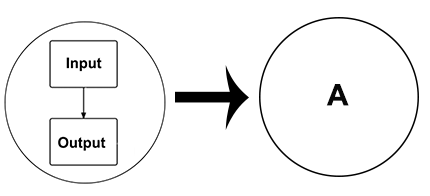
\includegraphics[width=.2\textwidth]{imgs/Nodo2.png}}
\caption{Abstração de uma transação como um vértice A.}
\label{vertice}
\end{figure}

 Considere então, o seguinte cenário, demostrado na figura : Se as transações Y e Y' reivindicarem fundos da transação X, somente uma das transações poderá ser publicada, Y ou Y", e assumimos então que elas estão em conflito. Supondo esta como a única restrição,  é possível representar em forma de grafo todas as transações, tendo as transações como vértices e  atribuindo arestas entre transações que estejam em conflito e dessa forma o minerador precisará encontrar o maior conjunto de vértices (transações) sem arestas entre eles (sem conflito). 
 
 \begin{figure}[ht]
\centerline{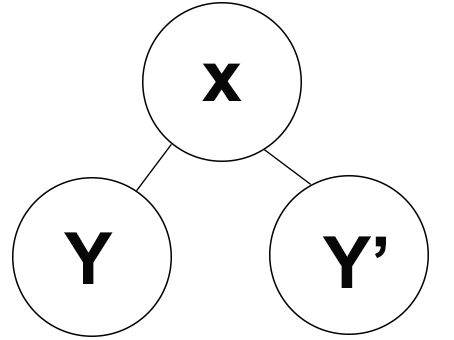
\includegraphics[width=.15\textwidth]{imgs/conflito.png}}
\caption{Cenário com transações conflitantes.}
\label{conflito}
\end{figure}

O problema do tipo gasto duplo acaba sendo um dos motivos de vulnerabilidades da rede de blockchain, gerando a possibilidade de vários ataques a rede. Vários ataques são conhecidos, dos quais podemos mencionar: Ataque de Corrida, Ataque Finney, Ataque Vector76,  Ataque de histórico alternativo e Ataque da majoritariedade.

Sendo assim, esse trabalho visa produzir uma alternativa de seleção de transações menos propensas a sofrer do problema do gasto duplo, pois não são provenientes de transações conflitantes para serem inseridas em um novo bloco minerado. Para isso, trata-se transações generalizadas contidas em forma de um grafo, onde vértices são as transações e as arestas são os conflitos existentes entre alguns vértices do grafo em questão.

Nós modelamos a rede Bitcoin como um grafo G = (V, E) e cada nó v corresponde a uma transação e assumimos que cada aresta \emph{e} $\in$ \emph{E} tem uma reivindicação de fundos associado a ela.


\section{Justificativa (ou demonstração) de o problema ser NP-difícil (ou NP-completo)}

Resolver isso é exatamente o problema do conjunto máximo independente. Mais uma vez, isso significa encontrar a solução ideal NP-hard e decidir se uma solução existe acima de um determinado tamanho (o que indicaria a taxa de transação total desde que assumimos taxas fixas de transação) é NP-completo.

Para se provar que um problema é NP-Completo são necessários dois passos:

\begin{enumerate}
    \item Mostrar que o problema pertence aos problemas NP.
    \item Mostrar que um problema NP-Completo conhecido pode ser polinomialmente redutível para ele.
\end{enumerate}

Levando em conta as considerações anteriores, será provado que criar um conjunto máximo de transações não conflitantes se trata de um problema NP-Completo, para um tamanho fixo $k$ de taxa de transação total.

\subsubsection{Prova de que pertence aos problemas NP}

A prova pode ser feita de duas formas:

\begin{itemize}
    \item Através de um algoritmo não determinístico polinomial para o problema (Algoritmo 1).
    \item Demonstrando que, a partir de uma solução para o problema, esta pode ser verificada em tempo polinomial.
\end{itemize}

\begin{algorithm}[htbp!]
\SetAlgoLined
\Entrada{$V$}
\Saida{Conjunto máximo de transações não conflitantes ($CMTNC$)}
\Inicio{
$i = 1$ \\
$CMTNC = inicializa\_cmtnc()$ \\
\ParaCada{$t \in V$}{
$j = escolhe(lista\_naoadj(i))$ \\
$i = j$ \\
$add\_cmtnc(CMTNC, j)$ \\
 }
}
\Retorna{$CMTNC$}
\label{alg:conjunto-maximo-transacoes-nao-deterministico}
\caption{\textsc{CMTNC Não determinístico}}
\end{algorithm}

Observando o Algoritmo 1, é definido uma transação inicial $i$ e para cada iteração $t$ menor ou igual ao conjunto de transações $V$, é escolhido uma transação $j$, não adjacente à $i$, e adicionado ao conjunto independente. Sendo assim, temos a iteração $t = {1 ... V}$ onde $V$ é o tamanho da entrada, problema já conhecido para o cálculo de complexidade de algoritmos, logo é possível determinar o algoritmo assintoticamente como $O(n)$.

\subsubsection{Prova de que o Maximum Independent Set é redutível para o Conjunto de Transações não Conflitantes}

\begin{figure}[htbp!]
\centerline{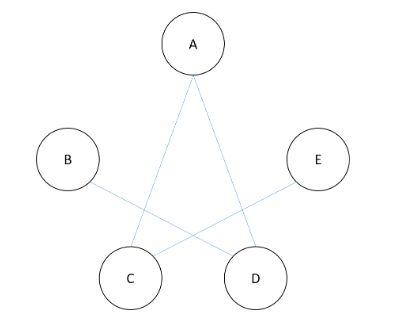
\includegraphics[scale=0.5]{imgs/grafo_mis.png}}
\caption{Grafo com 5 vértices e 4 arestas.}
\label{fig:grafo_mis}
\end{figure}

Considerando o grafo da Figura \ref{fig:grafo_mis} sendo uma instância para identificar conjuntos independentes, é possível determinar diferentes tipos:

\begin{itemize}
    \item Conjuntos independentes (CI): Todos conjuntos que consistem de vértices não adjacentes. p.ex $(A, E)$, $(E, D)$, $(C, D)$, $(B, C)$, $(B, E)$, $(A, B, E)$
    \item Conjuntos independentes máximos (CIM): $(E, D)$, $(C, D)$, $(B, C)$, $(A, B, E)$. Apesar do conjunto $(A, E)$ ser um conjunto independente, o mesmo não é um conjunto independente máximo devido ser subconjunto de $(A, B, E)$.
    \item Conjunto máximo independente (CMI): Entre todos os possíveis conjuntos independentes máximos, $(A, B, E)$ é o maior, portante é o conjunto máximo independente para o grafo.
\end{itemize}

Uma redução polinomial do CMI para o Conjunto Máximo de Transações não Conflitantes (CMTNC) pode ser feito da seguinte forma:

\begin{itemize}
    \item Para transações usa-se os vértices
    \item Para os conflitos entre transações usa-se as arestas (arestas adjacentes em nós representam tais conflitos)
\end{itemize}

Conforme citado na Seção \ref{subsec:descricao_formal_do_problema}, uma maneira de contornar transações conflitantes é encontrar o maior número de transações (vértices) que não se conflitam (não adjacentes).

É possível utilizar CMTNC para encontrar o conjunto máximo de transações não conflitantes que seja menor ou igual a $V$ (vértices). Sendo assim, o conjunto máximo é o CMI do grafo, $(A, B, E)$.

\section{Conjunto Independente}\label{CI}

Levando em consideração a teoria dos grafos, um Conjunto Independente (CI), também conhecido como conjunto estável, coclique ou anticlique, é um conjunto de vértices em um gráfico, dos quais dois não são adjacentes. Ou seja, é um conjunto \emph{S} de vértices tal que para cada dois vértices em \emph{S}, não existe arestas os conectando. 

Um CI de um grafo \emph{G} é um conjunto \emph{S} de vértices de \emph{G}, tal que não existem dois vértices adjacentes contidos em S. Em outras palavras, se \emph{a} e \emph{b} são vértices quaisquer de um conjunto independente, não há aresta entre \emph{a} e \emph{b}.

Por definição temos que todo grafo tem no mpinimo um CI: o conjunto vazio e um único grafo pode ter vários CIs distintos e o tamanho de um CI equivale ao número de vértices nele contido

Se \emph{S} é um CI de \emph{G} e não existe um CI de \emph{G} maior que \emph{S}, diz-se que \emph{S} é um CI máximo de \emph{G}. O problema de, dado um grafo \emph{G}, determinar se há um CI de tamanho k é um problema NP-completo.

Um CI máximo (\emph{ou  em inglês, Maximal Independent Set} é um CI, de forma que adicionar qualquer outro vértice ao conjunto força o conjunto a conter uma aresta ou o conjunto de todos os vértices do gráfico vazio.

Já o máximo de um CI (\emph{ou  em inglês, Maximum Independent Set} é um CI de maior tamanho possível para um dado gráfico \emph{G}. Esse tamanho é chamado de número de independência de \emph{G} e denotado $\alpha$(G). O problema de encontrar tal conjunto é chamado de problema do conjunto máximo independente e é um problema de otimização NP-difícil. Como tal, é improvável que exista um algoritmo eficiente para encontrar um conjunto independente máximo de um gráfico.

Todo conjunto máximo independente também é maximal, mas a implicação inversa não necessariamente se mantém.













\section{Revisão da Literatura}
Uma breve revisão da literatura foi realizada, conforme descrição da atividade, e assim vamos citar três trabalhos relacionados encontrados que tratam direta ou indiretamente da temática aqui proposta.

\subsection{Trabalhos Relacionados}

\subsubsection{Secure High-Rate Transaction Processing
in Bitcoin}

Este artigo, dos autores Yonatan Sompolinsky e Aviv Zohar, trata de uma investigação das implicações de segurança em se ter uma alta taxa de processamento de transações em Bitcoin contra ataques do tipo gasto duplo. É mostrado que em uma alta
taxa de transferência, os invasores substancialmente mais fracos são capazes de reverter os pagamentos que fizeram, mesmo depois de serem considerados aceitos pelos destinatários. 




\subsubsection{Handling Bitcoin Conflicts Through a Glimpse of
Structure}

Dois tópicos considerados principais pelos autores (Thibaut Lajoie-Mazenc, Romaric Ludinard e Emmanuelle Anceaume
) são abordados, são eles Gastos duplos e forks de blockchain, confrotando o sistema de criptografia Bitcoin. O primeiro se refere à habilidade do adversário de usar a mesma moeda mais de uma vez, enquanto a segunda reflete a ocorrência de inconsistências transitórias no histórico da estrutura de dados distribuída do blockchain. 



\subsubsection{Towards Risk Scoring of Bitcoin Transactions}

Aqui, os autores (Malte Moser, Rainer Bohme, and Dominic Breuker) demostram a preocupação em o Bitcoin se tornar o sistema de pagamento predominante na Internet e acreditam que supostos combatentes de crimes se unirão para regular e reforçar a lista negra de prefixos de transação nas partes que oferecem produtos reais e serviços em troca de bitcoin. 

Eles argumentam que Bitcoins na lista negra serão difíceis de serem gastos e, portanto, são menos valiosos. Assim sendo, acreditam que isso requer que todos os recebedores de pagamentos do Bitcoin não só verifiquem todas as listas negras de transações, mas também para avaliem o risco de uma transação na lista negra no futuro. 

\subsection{Técnicas Utilizadas}

No primeiro artigo, foi abordado a preocupação com a segurança através de métricas estabelecidas por meio da regra GHOST (The Greedy Heaviest-Observed Sub-Tree), uma modificação na forma como os nós Bitcoin constroem e reorganizam o cadeia de blocos, a estrutura de dados distribuída central do Bitcoin. O método GHOST foi adotado e uma variante dele foi implementada como parte de projeto em Ethereum, uma criptomoeda alternativa ao Bitcoin, uma plataforma de aplicações distribuídas de segunda geração. O modelo da rede Bitcoin é trazido na forma de um grafo orientado

Já no segundo artigo, os autores apresentam uma nova abordagem para enfrentar estas questões: adicionar algumas restrições à sincronização local de validação de transações do Bitcoin, e tornar essas restrições independentes do protocolo nativo da blockchain.  Restrições de sincronização são tratadas por nós da rede quee são escolhidos aleatoria e dinamicamente no sistema Bitcoin. Assim sendo, mostram que com tal abordagem, o conteúdo da blockchain é consistente com todas as transações validadas e blocos que garantem a ausência de ambos os ataques de gasto duplo e garfos blockchain. São feitas também análise de safety, liveness e not triviality do ecossistema Bitcoin. Assim como é apresentado um modelo de Orquestração de serviços de detecção de conflitos considerando os nós da rede Bitcoin e Tabelas de Hash Distribuidas. 

Por fim, o terceiro artigo traz a elaboração de um cenário, com um modelo de risco especificado, e a concepção de uma abordagem de previsão usando o conhecimento público apresentando resultados preliminares usando dados de roubos conhecidos selecionados. Os autores ainda discutem as implicações em mercados onde os bitcoins são negociados e trazem uma crítica sobre a capacidade do Bitcoin de servir como uma unidade de conta. É fornecido um Modelo de temporização da lista negra de transações com políticas diferentes (Poison, Haircut), assim como predição e análise de riscos e impacto.



\section{Metodologia}

Algumas abordagens podem ser utilizadas para o cálculo do CMTNC utilizando programação dinâmica, backtracking e algoritmos gulosos. O Algoritmo 2 descreve uma metodologia utilizando conceitos de algoritmos gulosos na tentativa de encontrar um ótimo global.

O algoritmo recebe como entrada um grafo $G(T,C)$ onde $T$ é o conjunto de transações (vértices) e $C$ o conjunto de conflitos (arestas). Cada transação $t_i$ possui um grau $d(t_i) \mid t_i \in T,\ i \in \mathbb{N}$, que é o número de conflitos existentes em uma transação, ou seja, a quantidade de vértices adjacentes a um vértice.

O algoritmo se inicia escolhendo uma transação $t_i$ de menor conflito $d(t_i) \forall t_i \in T$ adicionando-o ao conjunto máximo de transações não conflitantes $CMTNC$. Durante cada iteração é escolhido a próxima transação de menor conflito, podendo acontecer duas situações:

\begin{enumerate}
    \item A transação escolhida é realmente a menor
    \item $\exists$ duas menores transações com a mesma quantidade de conflitos
\end{enumerate}

Para a segunda opção é escolhida a transação de forma aleatória.

Em ambos casos é verificado se a nova transação $t_i \in CMTNC$, caso afirmativo, outra transação é escolhida, caso contrário, a transação é adicionada ao conjunto $CMTNC$ e removida do conjunto de transações $T$ (Algoritmo 2).

\begin{algorithm}[htbp!]
\SetAlgoLined
\Entrada{$G(T,C)$}
\Saida{Conjunto máximo de transações não conflitantes ($CMTNC$)}
\Inicio{
\Se{$T = \emptyset$}{
    \Retorna{$\emptyset$}
}
$CMTNC = inicializa\_cmtnc()$ \\
\Repita{$T = \emptyset$}{
$t = escolhe\_menor(T)$ \\
\Se{$t \notin CMTNC$}{
    $add\_cmtnc(CMTNC,\ t)$ \\
    $remove(T,\ t)$ \\
}
 }
}
\Retorna{$CMTNC$}
\label{alg:conjunto-maximo-transacoes}
\caption{\textsc{CMTNC}}
\end{algorithm}


%\subsection{Units}
%\begin{itemize}
%\item Use either SI (MKS) or CGS as primary units. (SI units are encouraged.) English units may be used as secondary units (in parentheses). An exception would be the use of English units as identifiers in trade, such as ``3.5-inch disk drive''.
%\item Avoid combining SI and CGS units, such as current in amperes and magnetic field in oersteds. This often leads to confusion because equations do not balance dimensionally. If you must use mixed units, clearly state the units for each quantity that you use in an equation.
%\item Do not mix complete spellings and abbreviations of units: ``Wb/m\textsuperscript{2}'' or ``webers per square meter'', not ``webers/m\textsuperscript{2}''. Spell out units when they appear in text: ``. . . a few henries'', not ``. . . a few H''.
%\item Use a zero before decimal points: ``0.25'', not ``.25''. Use ``cm\textsuperscript{3}'', not ``cc''.)
%\end{itemize}

%\subsection{Equations}
%Number equations consecutively. To make your 
%equations more compact, you may use the solidus (~/~), the exp function, or 
%appropriate exponents. Italicize Roman symbols for quantities and variables, 
%but not Greek symbols. Use a long dash rather than a hyphen for a minus 
%sign. Punctuate equations with commas or periods when they are part of a 
%sentence, as in:
%\begin{equation}
%a+b=\gamma\label{eq}
%\end{equation}

%Be sure that the 
%symbols in your equation have been defined before or immediately following 
%the equation. Use ``\eqref{eq}'', not ``Eq.~\eqref{eq}'' or ``equation \eqref{eq}'', except at 
%the beginning of a sentence: ``Equation \eqref{eq} is . . .''

%\subsection{\LaTeX-Specific Advice}

%Please use ``soft'' (e.g., \verb|\eqref{Eq}|) cross references instead
%of ``hard'' references (e.g., \verb|(1)|). That will make it possible
%to combine sections, add equations, or change the order of figures or
%citations without having to go through the file line by line.

%Please don't use the \verb|{eqnarray}| equation environment. Use
%\verb|{align}| or \verb|{IEEEeqnarray}| instead. The \verb|{eqnarray}|
%environment leaves unsightly spaces around relation symbols.

%Please note that the \verb|{subequations}| environment in {\LaTeX}
%will increment the main equation counter even when there are no
%equation numbers displayed. If you forget that, you might write an
%article in which the equation numbers skip from (17) to (20), causing
%the copy editors to wonder if you've discovered a new method of
%counting.

%{\BibTeX} does not work by magic. It doesn't get the bibliographic
%data from thin air but from .bib files. If you use {\BibTeX} to produce a
%bibliography you must send the .bib files. 

%{\LaTeX} can't read your mind. If you assign the same label to a
%subsubsection and a table, you might find that Table I has been cross
%referenced as Table IV-B3. 

%{\LaTeX} does not have precognitive abilities. If you put a
%\verb|\label| command before the command that updates the counter it's
%supposed to be using, the label will pick up the last counter to be
%cross referenced instead. In particular, a \verb|\label| command
%should not go before the caption of a figure or a table.

%Do not use \verb|\nonumber| inside the \verb|{array}| environment. It
%will not stop equation numbers inside \verb|{array}| (there won't be
%any anyway) and it might stop a wanted equation number in the
%surrounding equation.

%\subsection{Some Common Mistakes}\label{SCM}
%\begin{itemize}
%\item The word ``data'' is plural, not singular.
%\item The subscript for the permeability of vacuum $\mu_{0}$, and other common scientific constants, is zero with subscript formatting, not a lowercase letter ``o''.
%\item In American English, commas, semicolons, periods, question and exclamation marks are located within quotation marks only when a complete thought or name is cited, such as a title or full quotation. When quotation marks are used, instead of a bold or italic typeface, to highlight a word or phrase, punctuation should appear outside of the quotation marks. A parenthetical phrase or statement at the end of a sentence is punctuated outside of the closing parenthesis (like this). (A parenthetical sentence is punctuated within the parentheses.)
%\item A graph within a graph is an ``inset'', not an ``insert''. The word alternatively is preferred to the word ``alternately'' (unless you really mean something that alternates).
%\item Do not use the word ``essentially'' to mean ``approximately'' or ``effectively''.
%\item In your paper title, if the words ``that uses'' can accurately replace the word ``using'', capitalize the ``u''; if not, keep using lower-cased.
%\item Be aware of the different meanings of the homophones ``affect'' and ``effect'', ``complement'' and ``compliment'', ``discreet'' and ``discrete'', ``principal'' and ``principle''.
%\item Do not confuse ``imply'' and ``infer''.
%\item The prefix ``non'' is not a word; it should be joined to the word it modifies, usually without a hyphen.
%\item There is no period after the ``et'' in the Latin abbreviation ``et al.''.
%\item The abbreviation ``i.e.'' means ``that is'', and the abbreviation ``e.g.'' means ``for example''.
%\end{itemize}
%An excellent style manual for science writers is \cite{b7}.

%\subsection{Authors and Affiliations}
%\textbf{The class file is designed for, but not limited to, six authors.} A 
%minimum of one author is required for all conference articles. Author names 
%should be listed starting from left to right and then moving down to the 
%next line. This is the author sequence that will be used in future citations 
%and by indexing services. Names should not be listed in columns nor group by 
%affiliation. Please keep your affiliations as succinct as possible (for 
%example, do not differentiate among departments of the same organization).

%\subsection{Identify the Headings}
%Headings, or heads, are organizational devices that guide the reader through 
%your paper. There are two types: component heads and text heads.

%Component heads identify the different components of your paper and are not 
%topically subordinate to each other. Examples include Acknowledgments and 
%References and, for these, the correct style to use is ``Heading 5''. Use 
%``figure caption'' for your Figure captions, and ``table head'' for your 
%table title. Run-in heads, such as ``Abstract'', will require you to apply a 
%style (in this case, italic) in addition to the style provided by the drop 
%down menu to differentiate the head from the text.

%Text heads organize the topics on a relational, hierarchical basis. For 
%example, the paper title is the primary text head because all subsequent 
%material relates and elaborates on this one topic. If there are two or more 
%sub-topics, the next level head (uppercase Roman numerals) should be used 
%and, conversely, if there are not at least two sub-topics, then no subheads 
%should be introduced.

%\subsection{Figures and Tables}
%\paragraph{Positioning Figures and Tables} Place figures and tables at the top and 
%bottom of columns. Avoid placing them in the middle of columns. Large 
%figures and tables may span across both columns. Figure captions should be 
%below the figures; table heads should appear above the tables. Insert 
%figures and tables after they are cited in the text. Use the abbreviation 
%``Fig.~\ref{fig}'', even at the beginning of a sentence.

%\begin{table}[htbp]
%\caption{Table Type Styles}
%\begin{center}
%\begin{tabular}{|c|c|c|c|}
%\hline
%\textbf{Table}&\multicolumn{3}{|c|}{\textbf{Table Column Head}} \\
%\cline{2-4} 
%\textbf{Head} & \textbf{\textit{Table column subhead}}& %\textbf{\textit{Subhead}}& \textbf{\textit{Subhead}} \\
%\hline
%copy& More table copy$^{\mathrm{a}}$& &  \\
%\hline
%\multicolumn{4}{l}{$^{\mathrm{a}}$Sample of a Table footnote.}
%\end{tabular}
%\label{tab1}
%\end{center}
%\end{table}

%\begin{figure}[htbp]
%\centerline{\includegraphics{fig1.png}}
%\caption{Example of a figure caption.}
%\label{fig}
%\end{figure}

%Figure Labels: Use 8 point Times New Roman for Figure labels. Use words 
%rather than symbols or abbreviations when writing Figure axis labels to 
%avoid confusing the reader. As an example, write the quantity 
%``Magnetization'', or ``Magnetization, M'', not just ``M''. If including 
%units in the label, present them within parentheses. Do not label axes only 
%with units. In the example, write ``Magnetization (A/m)'' or ``Magnetization 
%\{A[m(1)]\}'', not just ``A/m''. Do not label axes with a ratio of 
%quantities and units. For example, write ``Temperature (K)'', not 
%``Temperature/K''.

%\section*{Acknowledgment}

%The preferred spelling of the word ``acknowledgment'' in America is without 
%an ``e'' after the ``g''. Avoid the stilted expression ``one of us (R. B. 
%G.) thanks $\ldots$''. Instead, try ``R. B. G. thanks$\ldots$''. Put sponsor 
%acknowledgments in the unnumbered footnote on the first page.

%\section*{References}

%Please number citations consecutively within brackets \cite{b1}. The 
%sentence punctuation follows the bracket \cite{b2}. Refer simply to the reference 
%number, as in \cite{b3}---do not use ``Ref. \cite{b3}'' or ``reference \cite{b3}'' except at 
%the beginning of a sentence: ``Reference \cite{b3} was the first $\ldots$''

%Number footnotes separately in superscripts. Place the actual footnote at 
%the bottom of the column in which it was cited. Do not put footnotes in the 
%abstract or reference list. Use letters for table footnotes.

%Unless there are six authors or more give all authors' names; do not use 
%``et al.''. Papers that have not been published, even if they have been 
%submitted for publication, should be cited as ``unpublished'' \cite{b4}. Papers 
%that have been accepted for publication should be cited as ``in press'' \cite{b5}. 
%Capitalize only the first word in a paper title, except for proper nouns and 
%element symbols.

%For papers published in translation journals, please give the English 
%citation first, followed by the original foreign-language citation \cite{b6}.

\begin{thebibliography}{00}
\bibitem{b1} Nakamoto, Satoshi. "Bitcoin: a peer-to-peer electronic cash system (2008).", 2008.
\bibitem{b2} Sompolinsky, Yonatan, and Aviv Zohar. "Secure high-rate transaction processing in bitcoin." International Conference on Financial Cryptography and Data Security. Springer, Berlin, Heidelberg, 2015.
\bibitem{b3} Lajoie-Mazenc, Thibaut, Romaric Ludinard, and Emmanuelle Anceaume. "Handling bitcoin conflicts through a glimpse of structure." Proceedings of the Symposium on Applied Computing. ACM, 2017.
\bibitem{b4} Möser, Malte, Rainer Böhme, and Dominic Breuker. "Towards risk scoring of Bitcoin transactions." International Conference on Financial Cryptography and Data Security. Springer, Berlin, Heidelberg, 2014.
\bibitem{b5}  "Bitcoin Wiki". En.Bitcoin.It, 2019, https://en.bitcoin.it/wiki/Main$_$Page. Accessed 1 June 2019.
\bibitem{b6} Cachin, Christian, et al. "The Transaction Graph for Modeling Blockchain Semantics.", IACR Cryptology ePrint Archive 2017 (2017): 1070.   
\end{thebibliography}
\vspace{12pt}

% \bibliographystyle{IEEEtran}
% \bibliography{bibtex}

\end{document}
